\section{HTML-Wanzen deaktivieren}
Bei HTML-Wanzen (sogenannten Webbugs) handelt es sich um 1x1-Pixel gro�e transparente Bildchen, welche in den HTML-Code einer Webseite oder einer E-Mail eingebettet werden. Sie sind f�r den Nutzer unsichtbar und werden beim Betrachten einer Webseite oder beim �ffnen der E-Mail von einem externen Server geladen.\\

Es ist relativ einfach, Webbugs zu deaktivieren indem das Laden der Grafiken von externen Servern unterbunden oder ein Content-Filter eingesetzt wird.\\

Einige Global Player im Internet (z.B. Ebay oder Amazon) verwenden externe Server f�r Grafiken und Bilder. F�r diese Server sind Ausnahmen zu definieren, um die Bedienbarkeit der Websites zu erm�glichen:

\begin{itemize}
 \item Ebay verwendet die Server \textit{ebayimg.com} f�r Bilder der angebotenen Produkte und \textit{pics.ebaystatic.com} f�r Navigationselemente.
\item Amazon verwendet den Server \textit{images-amazon.com} f�r die Coverbilder
\end{itemize}

\begin{figure}[htb]
\begin{center}
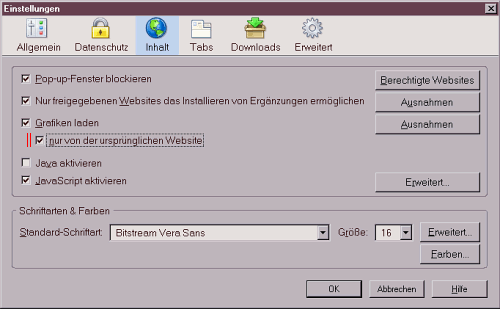
\includegraphics[scale=0.65]{../screenshots/firefox_grafiken.png}
\caption{Einstellungen zum Deaktivieren von HTML-Wanzen}
\label{abb:firefox_wanzen}
\end{center}
\end{figure}

\subsection{Firefox konfigurieren}
Im Browser Mozilla Firefox ist die entsprechende Option \textit{Grafiken nur von der urspr�nglichen Website laden} im Dialog \textit{Einstellungen} in der Sektion \textit{Inhalt} zu aktivieren (Bild \ref{abb:firefox_wanzen}). Damit werden die grafischen Linklisten vieler Websites leider etwas verunstaltet.\\

F�r einige Websites der Global Player wie Amazon oder Ebay sind Ausnahmen zu definieren. Ein Klick auf den Button \textit{Ausnahmen} �ffnet den im Bild \ref{abb:firefox_wanzen_ausn} gezeigten. Dialog. Hier k�nnen zul�ssige Server f�r das Laden von Grafiken definiert werden.

\begin{figure}[htb]
\begin{center}
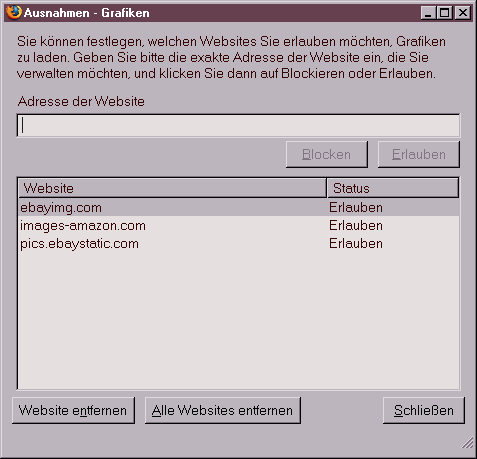
\includegraphics[scale=0.6]{../screenshots/firefox_grafiken_2.png}
\caption{Ausnahmen f�r das Laden von Grafiken}
\label{abb:firefox_wanzen_ausn}
\end{center}
\end{figure}
